\subsection{Class Diagram}


%Describe here the class diagram of your project



FinTrack is structured according to a three-tier architecture in which the business
logic layer acts as the mediator between the presentation and the data layers. This
layer is responsible for all domain-specific rules, input validation, and
computational logic of the application. It is composed of service classes, filter
classes, model objects, and data access objects, each with a clearly defined
responsibility. Service classes never communicate directly with the database; they
always delegate persistence to the appropriate DAO, keeping the business rules
independent of the underlying storage technology. The following subsections describe
each component category in detail.






\subsubsection{Servlets}


\begin{figure}[H]
    \centering
    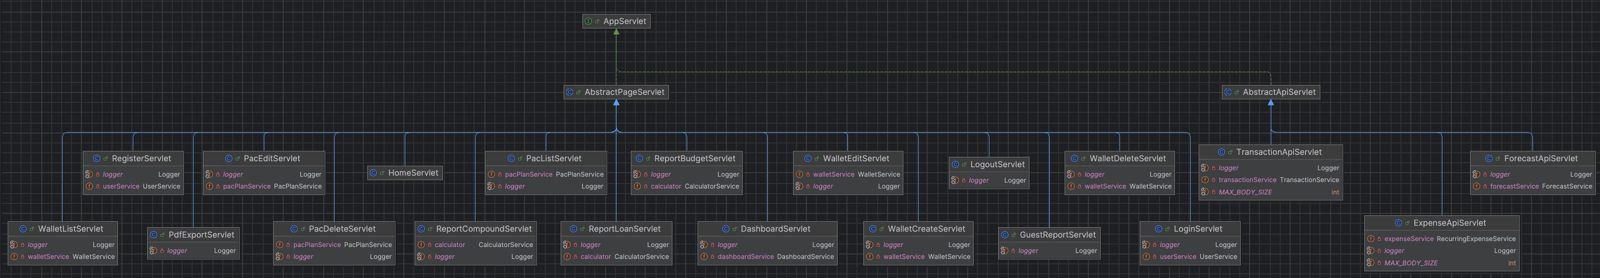
\includegraphics[width=0.9\textwidth]{sections/BLL/img/Servlet}
    \caption{Servlet diagram}
    \label{fig:servletdiagram}
\end{figure}


The application exposes two categories of servlets: page servlets, which follow the
Post/Redirect/Get pattern and produce HTML responses via JSP forwarding, and API
servlets, which accept and return JSON and serve AJAX-driven interactions on the
client side. Among the page servlets, \texttt{LoginServlet} and
\texttt{RegisterServlet} handle the two authentication entry points. Both accept
\texttt{POST} requests, delegate the operation to \texttt{UserService}, and on success create an authenticated
\texttt{HttpSession} via \texttt{AuthenticationSessionUtil} before redirecting the
user to the dashboard. On failure, they redirect back to the originating page with
an error code in the query string, which the corresponding \texttt{GET} handler of
the same servlet reads and translates into a user-facing message attribute before
forwarding to the JSP. \texttt{LogoutServlet} invalidates the current session and
redirects to the login page.
\texttt{DashboardServlet} loads the user's financial summary via
\texttt{DashboardService} and forwards the \texttt{DashboardSummary} object to the
dashboard JSP. \texttt{WalletListServlet} loads and displays all wallets;

\texttt{WalletCreateServlet}, \texttt{WalletEditServlet}, and
\texttt{WalletDeleteServlet} process the corresponding \texttt{POST} requests and
redirect with a \texttt{success} or \texttt{error} parameter. The same PRG pattern
is applied symmetrically by \texttt{PacListServlet}, \texttt{PacCreateServlet},
\texttt{PacEditServlet}, and \texttt{PacDeleteServlet} for investment plan management.
The guest area is served by \texttt{GuestReportServlet}, which displays the
calculator page, and by three calculator servlets: \texttt{ReportLoanServlet},
\texttt{ReportCompoundServlet}, and \texttt{ReportBudgetServlet}. Each of these
parses the submitted form parameters, calls \texttt{CalculatorService} to perform
the computation, serialises the result to JSON, and persists it into the guest
session via \texttt{ReportSessionDAO}. On validation failure, they re-forward to the
calculator JSP with an error message attribute rather than redirecting, so that the
user's input remains visible. \texttt{PdfExportServlet} handles PDF downloads for
both guest and authenticated users: for guests it validates the URL token against
the one stored in the \texttt{HttpSession} before generating the file, and for
authenticated users it fetches live dashboard data at download time.
The three API servlets --- \texttt{TransactionApiServlet},
\texttt{ExpenseApiServlet}, and \texttt{ForecastApiServlet} --- extend
\texttt{HttpServlet} and override the standard HTTP method handlers
(\texttt{doGet}, \texttt{doPost}, \texttt{doPut}, \texttt{doDelete}). Each servlet
extracts the resource identifier from the URL path using \texttt{getPathInfo()},
reads the JSON request body via a bounded \texttt{BufferedReader} (capped at 8~KB to
prevent abuse), deserialises it into a \texttt{JSONObject}, and delegates processing
to the corresponding service class. Errors are always returned as
\texttt{\{"error": "message"\}} JSON objects with the appropriate HTTP status code,
and a defensive session check provides a 401 response even if
\texttt{AuthenticationFilter} is somehow bypassed.



\subsubsection{Filters}

\begin{figure}[H]
    \centering
    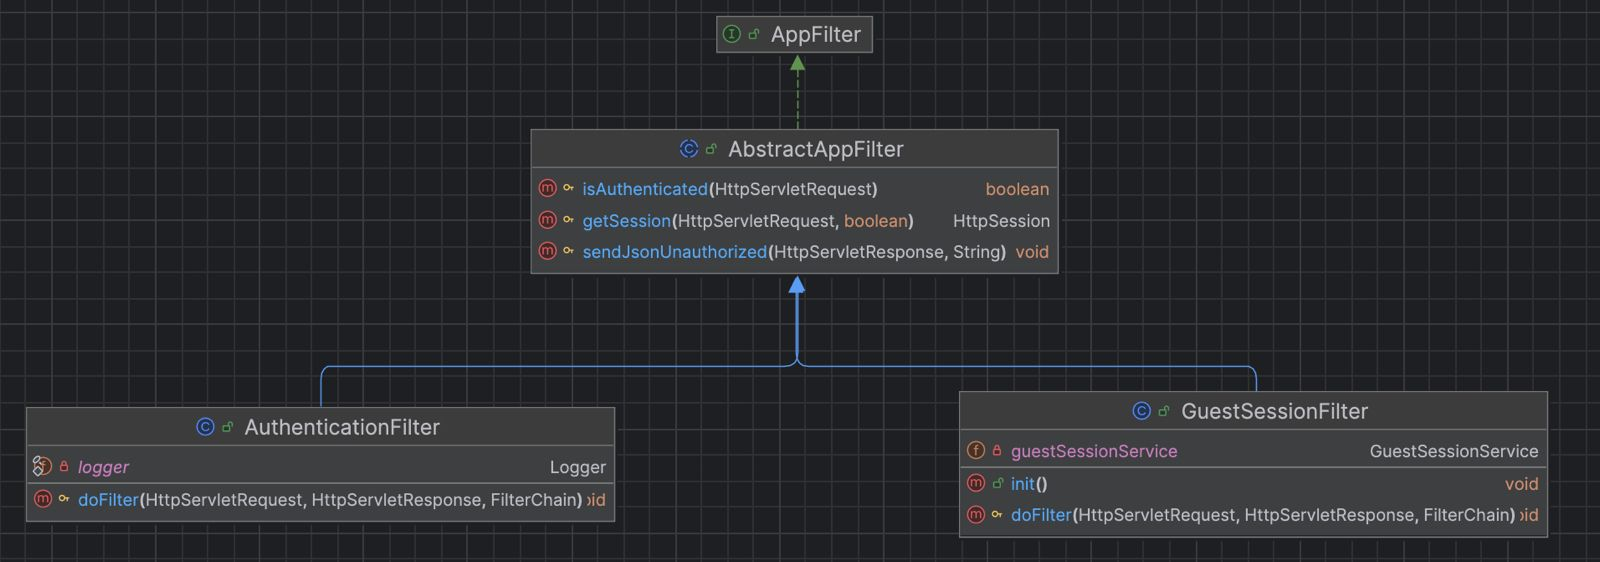
\includegraphics[width=0.8\textwidth]{sections/BLL/img/Filter}
    \caption{Filter diagram}
    \label{fig:filterdiagram}
\end{figure}

On our application we have two servlet filters govern access control for the entire application.
The first filter is \texttt{AuthenticationFilter} and is mapped to all routes that require a registered
account: \texttt{/dashboard}, \texttt{/wallets/*}, \texttt{/pac/*},
\texttt{/forecast/*}, \texttt{/transactions/*}, and \texttt{/api/*}. It checks
whether the current \texttt{HttpSession} contains an \texttt{authenticatedUser}
attribute. If not, it applies two different rejection strategies depending on the
request path: requests to \texttt{/api/*} receive a \texttt{401 Unauthorized} JSON
response (since those callers are JavaScript code and cannot follow a redirect),
while all other requests are redirected to \texttt{/login}.
The last filter is called \texttt{GuestSessionFilter} and mapped to the guest calculator routes
(\texttt{/guest/*}, \texttt{/report/loan}, \texttt{/report/compound},
\texttt{/report/budget}). It ensures that every visitor has an active guest session
before reaching the servlet, creating one transparently if needed. It reads the
\texttt{guestSessionToken} attribute from the \texttt{HttpSession}, delegates to
\texttt{GuestSessionService.ensureGuestSessionExists()}, and stores the returned
token back into the session. The service handles both the case where no token exists
yet and the case where the token's database row has expired, creating a fresh session
in both cases.


\subsubsection{Resources}

\begin{figure}[H]
    \centering
    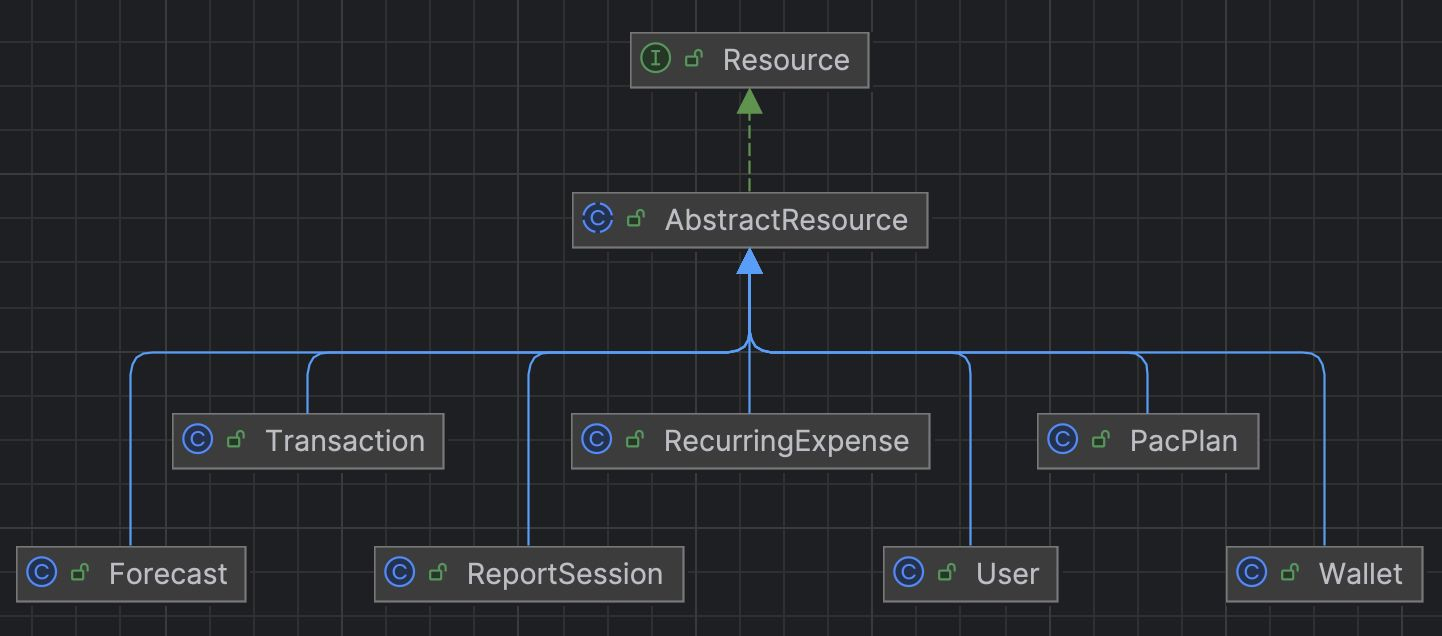
\includegraphics[width=0.8\textwidth]{sections/BLL/img/Resources}
    \caption{Resources diagram}
    \label{fig:Resourcesdiagram}
\end{figure}

The model package contains the data transfer objects and domain entities shared
across all layers. \texttt{User} stores the user's identity and PBKDF2 password hash.
\texttt{Wallet} holds the name, type, and currency of a financial account.
\texttt{Transaction} records a single financial movement, storing the absolute amount
alongside an explicit \texttt{TransactionType} enum (\texttt{INCOME} or
\texttt{EXPENSE}). \texttt{RecurringExpense} describes a periodic fixed cost linked
to a wallet, with a \texttt{Periodicity} enum (\texttt{MONTHLY}, \texttt{QUARTERLY},
\texttt{YEARLY}) and an active/inactive flag. \texttt{PacPlan} holds a PAC investment
plan with a monthly contribution and a target amount.
Several read-only value objects are produced by the analytics layer.
\texttt{WalletSummary} carries a computed balance alongside the wallet metadata.
\texttt{DashboardStats} is a Java record holding per-currency equity, YTD expenses,
and YTD savings. \texttt{DashboardSummary} wraps both collections into a single
object for the presentation layer. \texttt{Forecast} stores the scenario name and
the 24-entry projection JSON array.
The guest area uses three result objects specific to \texttt{CalculatorService}:
\texttt{AmortizationRow} (one row per month of the loan schedule),
\texttt{CompoundResult} (one entry per year of the compound interest projection),
and \texttt{BudgetResult} (income and expense totals with per-category breakdowns).
\texttt{ReportSession} holds the guest's accumulated JSON payload alongside its
expiry timestamp.



\subsubsection{Data Access}

\begin{figure}[H]
    \centering
    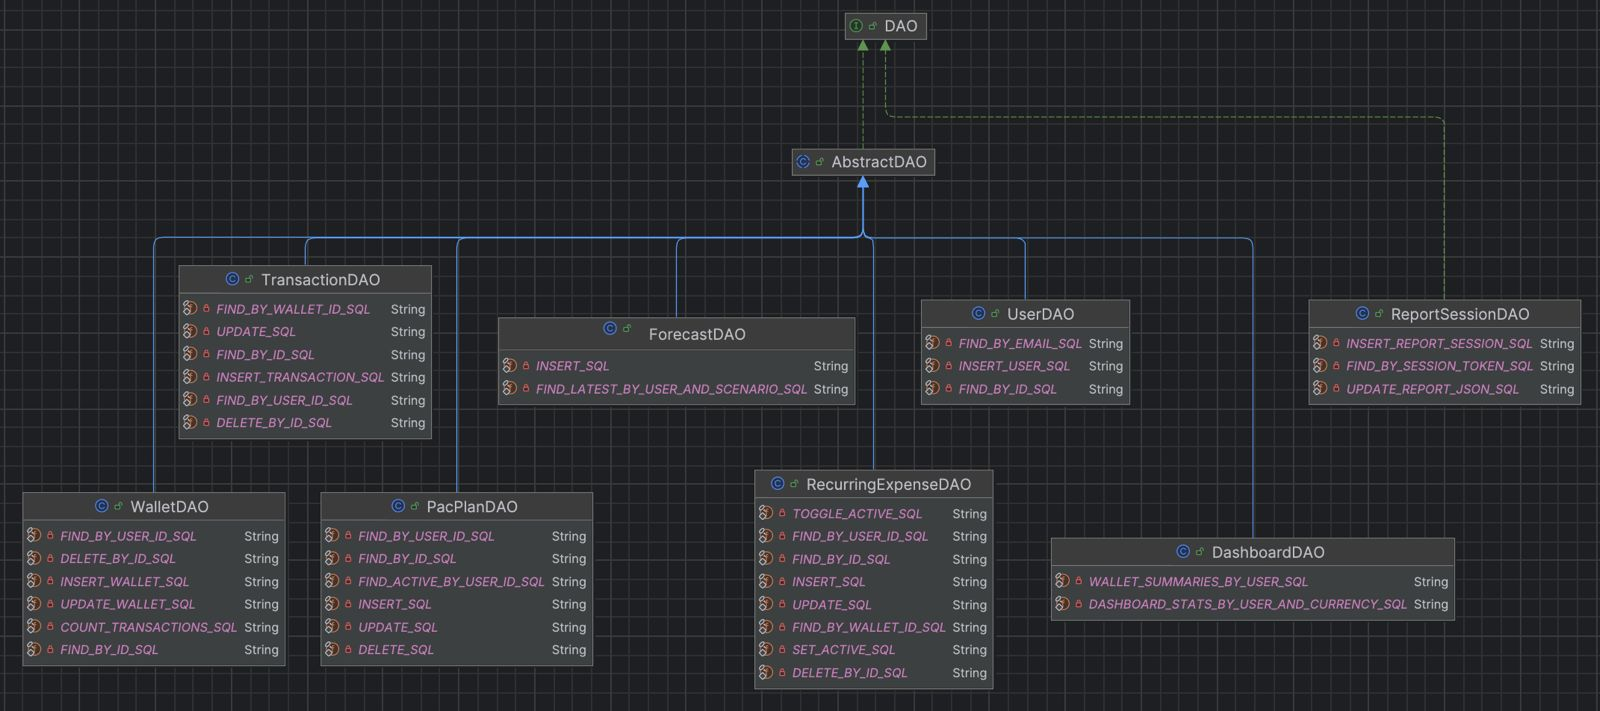
\includegraphics[width=0.8\textwidth]{sections/BLL/img/Dao}
    \caption{DAO diagram}
    \label{fig:daodiagram}
\end{figure}

Each service class depends on one or more DAO classes that encapsulate all database
interaction. Every DAO opens connections via a shared \texttt{DBConnection} utility
and uses \texttt{try-with-resources} to ensure that connections, statements, and
result sets are always closed, even on exceptional paths. SQL queries are held in
\texttt{private static final String} constants and executed exclusively through
\texttt{PreparedStatement}, eliminating any risk of SQL injection.
\texttt{UserDAO} provides lookup by email and user creation. \texttt{WalletDAO}
supports full CRUD operations and exposes a \texttt{countTransactions()} method used
by the service to enforce the no-deletion-with-transactions rule.
\texttt{TransactionDAO} adds a \texttt{findByUserId()} method used by
\texttt{ForecastService} to reconstruct the historical balance.
\texttt{RecurringExpenseDAO} provides both a per-wallet and a per-user lookup to
support the expense management page and the forecast computation respectively.
\texttt{PacPlanDAO} exposes a \texttt{findActiveByUserId()} method for the same
reason. \texttt{DashboardDAO} executes two aggregation queries: one that computes
per-wallet running balances via conditional \texttt{SUM(CASE WHEN ...)} expressions,
and one that produces per-currency YTD statistics using the same technique filtered
by the current year. \texttt{ForecastDAO} stores projections and retrieves the most
recent one per user and scenario via \texttt{ORDER BY created\_at DESC LIMIT 1}.
\texttt{ReportSessionDAO} manages guest session rows, including creation with an
expiry timestamp and JSON update; the expiry check is enforced at the query level
by appending \texttt{AND expires\_at > CURRENT\_TIMESTAMP} to the lookup condition.



\subsubsection{REST Resources and Routing}

\begin{figure}[H]
    \centering
    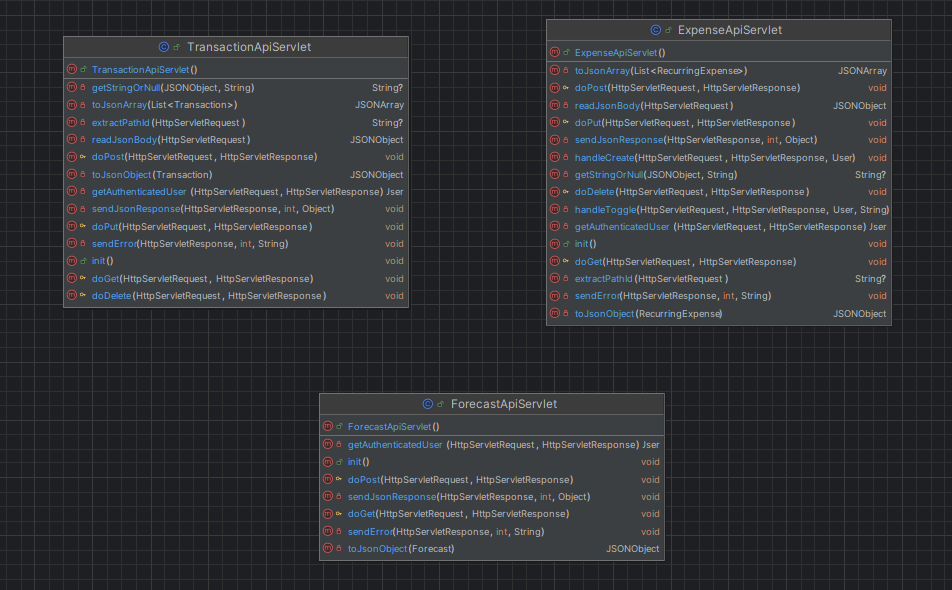
\includegraphics[width=0.6\textwidth]{sections/BLL/img/api_servlet}
    \caption{Api diagram}
    \label{fig:apidiagram}
\end{figure}

The application exposes its REST interface under the \texttt{/api/} prefix, which is
protected uniformly by \texttt{AuthenticationFilter}. Resources are addressed with
RESTful URL patterns and method semantics.
\texttt{/api/transactions/*} is handled entirely by \texttt{TransactionApiServlet}.
The path segment after the prefix, extracted via \texttt{getPathInfo()}, identifies
the individual transaction for \texttt{PUT} and \texttt{DELETE} operations, while
\texttt{GET} uses a \texttt{walletId} query parameter to return all transactions
belonging to a wallet. \texttt{POST} creates a new transaction from a JSON body
containing the wallet identifier, amount, category, date, and an optional note.
\texttt{/api/expenses/*} follows the same structural pattern via
\texttt{ExpenseApiServlet}, with the addition of a sub-resource path:
\texttt{/api/expenses/\{id\}/toggle} accepts a \texttt{POST} request to flip the
active status of a recurring expense without requiring a full update payload.
\texttt{/api/forecast} is served by \texttt{ForecastApiServlet}. A \texttt{POST}
request with a \texttt{scenario} query parameter triggers a full recomputation and
stores the result; a \texttt{GET} request retrieves the latest stored projection for
the same scenario. The three valid scenario values --- \texttt{OPTIMISTIC},
\texttt{CONSERVATIVE}, and \texttt{STRESS\_TEST} --- are resolved via
\texttt{ForecastScenario.valueOf()}, and an \texttt{IllegalArgumentException} from
that call is mapped to a \texttt{400 Bad Request} response.

























